\documentclass[11pt,a4paper]{article}

\usepackage{classeRapport}

\begin{document}

   
    \PageDeGarde
    {Image-snake.jpg}
    {Rapport projet I4}
    {Création du jeu snake}
    {Kévin \textsc{Gatel}\\
    Julien \textsc{Gavaud}\\
    Hengshuo \textsc{LI}\\
    Simon \textsc{Morin}\\
    Yizhe \textsc{Wang}\\
    Théo \textsc{Willekens}} 
    {I4-2 – STPI-2 – 2019-2020}
    
    \Page{INSALogo}
    
    \tableofcontents

    \clearpage 

    \vspace*{\stretch{1}}

        \section*{Introduction}
        \addcontentsline{toc}{section}{Introduction} 
        
        \vspace{1cm} 
        
        Au cours de notre formation au sein de l'INSA ou plus tard dans le monde du travail nous serons amener à réaliser des projets. Que ce soit des projets d'informatiques ou non il nous faudra non seulement de solides connaissances mais également une bonne organistaion pour les mener à bien. Savoir gérer un projet cela s'apprend. L'enseignement d'I4-2 dispensé au sein de l'INSA a pour but de nous initier à la gestion de projet. Pour cela rien de mieux que la pratique. Nous avons donc mener un projet informatique en groupe (6 personnes). Ce rapport en présente les différentes étapes. Le but de ce projet est double. Dans un premier temps il vise à nous familiariser avec l’outil git, qui est un logiciel de gestion de versions décentralisé. Dans un second temps, l’objectif est d’utiliser nos connaissances en informatique et de continuer à les développer pour réussir à coder le jeu « snake ».

        \vspace*{\stretch{1}}

        \clearpage 

    \section{Analyse du projet}

    \subsection{Cahier des charges}
        \subsubsection{Description du projet}
             L'objectif de ce projet est donc de coder le jeu ``snake'', bien connu de tous. Pour faciliter le travail, nous allons utiliser l'outil git. Cependant, laissant libre cours à notre imagination, ce projet ne vise pas à reproduire le célèbre jeu mais bien à créer notre version inédite. Pour cela, une bonne organisation au sein du groupe est nécessaire. Nous nous sommes ainsi réunis en amont pour définir toutes les options que l'on ajouterait à ce jeu. L’outil git va par ailleurs nous être particulièrement utile. Bien utilisé, il nous permettra un bon suivi du travail, tout en permettant à chacun de travailler à son rythme. Concernant la partie programmation, le ``snake'' sera codé en Pascal. 
        
        \subsubsection{Description du jeu}
            Le principe du jeu est simple. Un serpent est enfermé dans une cage, dont il ne peut pas sortir. La cage est symbolisée par une map rectangulaire, fermée par des murs. Le but du jeu est d’avoir un maximum de points. Pour cela, le serpent doit manger des pommes qui apparaissent sur la map aléatoirement. A chaque pomme mangée, le score est implémenté. Pour que le jeu ait un intérêt, plus le serpent mange de pommes, plus il grandira. Il devient donc de plus en plus dur de diriger le serpent. Par ailleurs, si la tête du serpent touche sa queue (le reste de son corps) celui-ci meurt. Il meurt également s'il touche les murs qui délimitent la map. Si le serpent meurt, la partie s'arrête. 
            
        \subsubsection{Liste des fonctionnalités}\label{sssect:fonctionnalites}
            Le rendu final de notre projet comportera les fonctionnalités suivantes:
            \begin{itemize}
            
                \item Permettre de modifier la trajectoire du serpent (droite/gauche/haut/bas) avec les flèches du clavier.
                \item Des pommes apparaissent sur la map et la taille du serpent s’incrémente à chaque fois qu’il mange une pomme.  
                \item Comptage des scores (en relation avec la taille du serpent) pour donner une dimension \enquote{compétitive} au jeu. 
                \item Le jeu s’arrête si la tête du serpent rencontre un mur/obstacle ou sa queue.
                \item Affichage graphique grâce à la \textit{SDL}.
                \item Mise en place d'un menu à choix multiples permettant de changer le niveau de difficulté entre autres.
                
            \end{itemize}


        \clearpage
        
        Nous avons prévu des fonctionnalités \underline{optionnelles}, qui ne seront implémentées que s'il nous reste du temps à la fin du semestre:
            \begin{itemize}
            
                \item Ajout d’une pomme dorée à durée de vie courte qui 
                donnerait, si elle est mangée, des points bonus au joueur. Elle pourrait aussi déclencher des actions « extraordinaires » comme le passage d’un mur à l’autre ou bien faire accélérer le serpent ponctuellement. 
                \item Sauvegarde des scores permettant la création d'un 
                classement.
                \item Ajout d’obstacles sur la map (ex : colonne à ne pas 
                toucher ou pots de fleurs). Le serpent devra alors réussir à les esquiver. Leur fonctionnement serait différent de ceux des murs au sens que si le serpent les touche, il ne meurt pas mais le joueur perd des points et la taille du serpent diminue. Si le serpent a perdu "toute sa taille" alors la partie s'arrête. 
                \item Les pommes apparaissent de manière intelligente. Plus le joueur possède de    points plus celles-ci apparaissent près des murs ou des obstacles. 
                \item Ajout d'un timer pour créer un sytème de comptage de points alternatifs et changer la vitesse du serpent en fonction de la durée de la partie pour la pimenter.
                \item Différents choix de map possibles (circulaire,carré...).
               
            \end{itemize}
            

    \subsection{Prévision des livrables}
        
        \textbf{Versions prévues :}
        
        \vspace{0.5 cm}
        V1 (02/04/2020):
        \begin{itemize}
        
            \item Affichage map, pomme, obstacle et serpent. Mouvement du 
                  serpent en ligne droite. Meurt quand il touche un mur. L'utilisateur peut 
                  modifier la trajectoire du serpent pour le faire tourner à gauche ou à droite.
            \item Recherche de fluidité.
            
        \end{itemize}
        
        \vspace{0.3 cm}
        V2 (09/04/2020):
        \begin{itemize}
        
            \item Le serpent grandit quand il mange une pomme. Il rétrécit quand il rencontre un obstacle.
            
        \end{itemize}
        
        \vspace{0.3 cm}
        V3 (14/05/2020):
        \begin{itemize}
        
             \item Ajout d'un compteur de points en relation avec la taille du serpent. 
             \item Ajout d'un bonus (pomme dorée) qui apparaît à l'écran tous les 100 points et qui permet d'accélérer les mouvements du serpent. Ce bonus est à durée limitée.
             \item Ajout d'un menu pour choisir la taille de la map, et ainsi changer la difficulté.
             \item Ajout d'un fichier des meilleurs scores (si l'utilisateur fait un des 3 meilleurs scores, son score sera sauvegardé et intégré). 
            \item Version \textit{SDL}
            
        \end{itemize}
        
        \vspace{0,5 cm}
        
        \textbf{Version finale (24/05/2020)}
        \begin{itemize}
        
             \item Rendu du rapport
             \item Rendu du code source complet et de la conception détaillée des fonctions et procédures les plus importantes. 
             
        \end{itemize}

    \subsection{Conception globale}
        Cette section présente la conception globale du programme implémentant les fonctionnalités données en section~\ref{sssect:fonctionnalites}.
        L'analyse descendante correspondante est donnée par les figures 1, 2 et 3 ci-dessous.
        
        \subsubsection{Analyse descendante}
            Cette première figure montre la première échelle de notre programme. On voit la partie principale permettant de créer notre jeu Snake.
            
            \begin{figure}[!ht]
            
                \centering 
                \includegraphics[width=1\textwidth]{images/AD_1.pdf} 
                \caption{Analyse descendante du projet - partie 1.} 
                \label{fig:AD} 
                
            \end{figure}
            
            \clearpage
            \par
                Nous observons ici notre deuxième partie, représentant la suite de cette analyse descendante, en entrant dans la partie plus précise.    
            
            \begin{figure}[!ht]
            
                \centering 
                \includegraphics[width=1\textwidth]{images/AD_2.pdf} 
                \caption{Analyse descendante du projet - partie 2.}
                \label{fig:AD} 
                
            \end{figure}
            
            \clearpage
            \par
                Enfin, nous retrouvons le détail de la procédure Déplacement, une procédure essentielle à notre programme. Le détail des appels utilisés dans cet procédure permet de comprendre la structure et la logique de notre code.
            
            \begin{figure}[!ht]
            
                \centering 
                \includegraphics[width=1\textwidth]{images/AD_3.pdf} 
                \caption{Analyse descendante du projet - partie 3.} 
                \label{fig:AD} 
                
            \end{figure}    
        
        \clearpage
    
        \subsubsection{Conception préliminaire}
        Le contenu de cette sous-section présente les types que nous avons utilisé pour programmer notre jeu.
        Cette section contient également la signature des fonctions et procédures de l'analyse descendante, en précisant les entrées, sorties et entrées/sorties.

            \begin{lstlisting}[language=Pascal,frame=single,caption=Principaux types utilisés.]
Type coordonnee = record
        x : Integer;
        y : Integer;
                end;                  
                    
tableau2D = array[1..longueur,1..largeur] of String;

tableau_obstacle = array[1..max_obstacle] of coordonnee;	

tableau_snake = array[1..longueur*largeur] of coordonnee;

tableaudirection = array[1..longueur*largeur] of String;

            \end{lstlisting}

            \textbf {Commentaires : } 
                \begin{itemize}
                    \item Le type coordonnee permet d'accéder aux positions sur la grille de jeu (la map) des différents élèments. 
                    \item Le type tableau2D est le support principal du jeu. Il permet de "créer" une grille dans laquelle sera mise toutes les informations relatives à la map pour pouvoir les afficher et les adapter au cours du jeu (comme la position des pommes ou du serpent).
                    \item Le tableaudirection est le type qui a été créé pour retenir les positions du serpent en entier. Pour afficher le serpent en \textit{SDL} nous avons 4 images pour la tête, le corps et la queue (12 au total) une dans chaque direction (si le serpent va de gauche à droite ou de droite à gauche par exemple). Le tableaudirection nous permet de gérer le choix de ces images. 
                    \item Le tableau\_snake permet de  garder en mémoire les coordonnées de chaque "morceau" du serpent sur le terminal. Cela permet ensuite de générer par exemple des coordonnées pour les pommes différentes du serpent.
                    \item Pour pouvoir accéder plus facilement aux coordonnées des différents éléments, nous avons utilisé les 3 fonctions ci-dessous. Elles permettent également plus de flexibilité et une meilleure lisibilité. 
                \end{itemize}
            
            \begin{lstlisting}[language=Pascal,frame=single,caption=Signatures des procédures de l'unité types]
function x(xy : coordonnee) : integer;

function y(xy : coordonnee) : integer;

procedure fixer_xy(var xy : coordonnee; valeurx,valeury : Integer);
            
            \end{lstlisting}

            \clearpage
            \begin{lstlisting}[language=Pascal,frame=single,caption=Signatures des procédures du programme principal snakee]
procedure initmap(E/S tab: tableau2D; S pomme: coordonee;
            S obstacle:tableau_obstacle; 
            S nbre_obstacle,obstacle_rencontres: integer;
            E difficulte: integer)
            
procedure initsnake(S tab: tableau2D; S tabdirection: tableaudirection;
            S i_snake: tableau_snake; E/S taille_snake: integer; 
            S direction: string; E difficulte: integer)
            
procedure partie(E/S perdu: boolean; E difficulte: integer)
            
procedure navigation_menu(E/S exit,perdu: boolean)
            
            \end{lstlisting}

            \begin{lstlisting}[language=Pascal,frame=single,caption=Signatures des procédures de l'unité création]
procedure creationpomme(E/S tab: tableau2D; S pomme: coordonnee; 
                E difficulte: integer; E normalOuDoree : string)
            
procedure creationObstacle(E/S tab:tableau2D; S obstacle:tableau_obstacle; 
            E/S nbre_obstacle: integer; S coord: coordonnee;
            E difficulte: integer)
            
procedure afficherTab(E tab: tableau2D);
            
function genererCoordonnee(E tab:Tableau2D; 
E difficulte:integer):coordonnee;
                
            \end{lstlisting}

            \begin{lstlisting}[language=Pascal,frame=single,caption=Signatures des procédures de l'unité menu]
procedure affichage_Menu();
            
procedure regleJeu();
            
procedure creditsJeu();
            
function choix_diff() : integer;
            
            \end{lstlisting}

            \textbf {Commentaires : } 
                \begin{itemize}
                
                    \item Ces procédures gèrent simplement l'affichage texte du menu. Elles permettent de charger des fichiers textes pour ensuite les afficher à l'écran dans les différentes options du menu. 
                    
                \end{itemize}
                
            \clearpage
            
            \begin{lstlisting}[language=Pascal,frame=single,caption=Signatures des procédures de l'unité ranking]
procedure ranking(E pommes_mangees, E pommesdorees_mangees,
            E obstacles_rencontres : Integer);
            
procedure affichranking();
            
            \end{lstlisting}

            \begin{lstlisting}[language=Pascal,frame=single,caption=Signatures des procédures de l'unité deplacement]
procedure deplacement(E/S tab: Tableau2D
            E/S tabdirection: tableaudirection
            E/S snake : tableau_snake
            E/S obstacle : tableau_obstacle
            E/S direction : string
            E/S perdu,echap : boolean
            E/S taille_snake,pommes_mangees,
            pommesdorees_mangees,obstacles_rencontres,
            nbre_obstacle,vitesse_init: integer
            E/S casesParcourues : Longint
            E/S pomme,pommedoree:coordonnee
            E/S difficulte : integer
            E/S pommedodovf,murgold: boolean)
                                  
procedure lignedroite(E/S tab: Tableau2D; 
            E direction: string
            E ms : integer)
            E/S tabdirection: tableaudirection
            E/S snake: tableau_snake
            E/S obstacle: tableau_obstacle
            E/S taille_snake, pommes_mangees,
            pommesdorees_mangees, 
            obstacles_rencontres,nbre_obstacle : integer
            E/S casesParcourues : Longint
            E/S pomme,pommedoree : coordonnee
            E/S perdu : boolean
            E/S difficulte,vitesse_init : integer
            E/S pommedodovf,murgold: Boolean
                                    
procedure changementDirection(E k_string: string; E/S direction: string )
            
            \end{lstlisting}

            \clearpage
            
            \begin{lstlisting}[language=Pascal,frame=single]
procedure rencontrer_pomme(E/S tab: Tableau2D
            E/S  tabdirection: tableaudirection
            E/S  snake: tableau_snake
            E/S  obstacle: tableau_obstacle
            E/S  direction: string
            E/S  pomme: coordonnee
            E/S  taille_snake,nbre_obstacle,pommes_mangees, 
            pommesdorees_mangees, obstacles_rencontres : Integer
            E  mem_queue : coordonnee 
            E  symbole: string
            E/S  difficulte: integer)
            
procedure rencontrer_obstacle(E/S  tab: Tableau2D; 
            E/S  tabdirection: tableaudirection; 
            E/S  snake: tableau_snake; 
            E/S  obstacle: tableau_obstacle; 
            E/S  taille_snake,pommes_mangees, pommesdorees_mangees,
            obstacles_rencontres,
            nbre_obstacle: Integer
            E/S  perdu: boolean;
            E/S  difficulte: integer) 
            
procedure rencontrer_snake(E/S  perdu: boolean) 
            
procedure rencontrer_mur(E/S  perdu: boolean) 
            
procedure rencontrer_pommedoree(E/S  tab: Tableau2D
            E/S  snake: tableau_snake
            E/S  pommedoree: coordonnee
            E/S  pommes_mangees,pommesdorees_mangees, 
            obstacles_rencontres, difficulte,vitesse_init: integer
            E/S  casesParcourues: Longint
            E/S  pommedodovf,murgold: boolean)
                                            
function directionValide(E k_string, E direction : string): boolean;
            
function score(E pommes_mangees, E pommesdorees_mangees, 
            E obstacles_rencontres : Integer) : Integer;                                 
            \end{lstlisting}
            
            \clearpage

    \subsection{Conception détaillée}
        Cette partie nous permet de présenter en détail quelques-unes de nos procédures les plus complexes et interressantes en pseudo-code. Pour les réaliser sur \LaTeX{}, nous avons utiliser le paquet spécifique algorithm2e
        
        \vspace{0,5 cm}
        
        \begin{algorithm}[H]
            \SetAlgoLined
            \Proc{partie(E/S perdu: Booléen; E difficulte: Entier)}{
            \Sortie{La partie est lancée et tant que le booléen perdu est faux le joueur peut continuer à jouer}
            \Donnees{
            tab : tableau2D \; 
            snake : tableau\_snake \; 
            taille\_snake, nbre\_obstacle, pommes\_mangees, pommesdorees\_mangees, obstacles\_rencontres, vitesse\_init : Entier\; 
            perdu, echap : Booléen ; direction : Chaîne de caractères \; 
            pomme : coordonnee ; obstacle : tableau\_obstacle }
            
            \Deb{
        
            initmap(tab, pomme, obstacle, nbre\_obstacle, obstacles\_rencontres, difficulte)\;
            initsnake(tab, pomme, obstacle, nbre\_obstacle, obstacles\_rencontres, difficulte)\;
            init\_sdl(difficulte) / init\_gif(tabgif) / afficherTab(tab)\;
            \tcp{On gère la vitesse du serpent :}
            vitesse\_init $\leftarrow$ vitesse\_initiale;
            delay(vitesse\_init)\;
            \tcp{Toutes les variables sont initialisées en début de partie comme par exemple : (on ne les note pas toutes ici)}
            pommes\_mangees $\leftarrow$ 0\;
            afficher\_score(scr, difficulte)\;
            
            \Tq{(perdu = Faux) et (echap = Faux)}{
            deplacement(tab, tabdirection, snake, obstacle, ..., difficulte, pommedodovf, murgold)\;
            \tcp{Tous les paramètres n'ont pas été notés pour ne pas alourdir la présentation (pour plus de précisions, se référer à l'algorithme 3)}
            casesParcourues $\leftarrow$ casesParcourues + 1\;
            }
            \tcp{Si le joueur a perdu, on affiche l'image de fin et le classement en fonction de son score :}
            \Si{perdu = Vrai}{game\_over()\;}
            free\_sdl()\;
            ranking(pommes\_mangees, pommesdorees\_mangees, obstacles\_rencontres)\;
            }
            }
            \caption{Permet de regrouper les différentes procédures pour lancer une partie}
        \end{algorithm}
        
% Problème de saut de page entre les algorithmes qui donnait des pages blanches inutilement

\begin{minipage}{1cm}
 
\end{minipage}

        \begin{algorithm}[H]
            \SetAlgoLined
            \Proc{lignedroite (E/S tab : Tableau2D; E snake : tableau\_snake; E/S obstacle : tableau\_obstacle; E/S taille\_snake, pommes\_mangees, obstacles\_rencontres, nbre\_obstacle : Entier; E/S perdu : Booléen; E direction : Chaîne de caractères; E pomme : coordonnee)}{
            \Sortie{On aura les procédures 'rencontrer\_' qui seront activées en fonction du déplacement du serpent}
            \Donnees{indice\_x, indice\_y, i : Entier; symbole, cqueLaQueueRencontre : Chaîne de caractère; mem\_queue : coordonnée}
            
            \Deb{
            \Switch{direction}{
            \uCase{'right'}{
            indice\_x $\leftarrow$ 1;
            indice\_y $\leftarrow$ 0;
            symbole $\leftarrow$ '>'\;
            }
            \uCase{'left'}{
            indice\_x $\leftarrow$ -1;
            indice\_y $\leftarrow$ 0;
            symbole $\leftarrow$ '<'\;
            }
            \uCase{'up'}{
            indice\_x $\leftarrow$ 0;
            indice\_y $\leftarrow$ 1;
            symbole $\leftarrow$ 'n'\;
            }
            \uCase{'down'}{
            indice\_x $\leftarrow$ 0;
            indice\_y $\leftarrow$ -1;
            symbole $\leftarrow$ 'v'\;
            }
            }
            cqueLaQueueRencontre $\leftarrow$ tab[x(snake[1]) + indice\_x, y(snake[1]) + indice\_y]\;
            \tcp{Atttribue les entrées aux coordonnées de mem\_queue}
            fixer\_xy(mem\_queue, x(snake[taille\_snake]), y(snake[taille\_snake]))\;

            tab[x(snake[1]) + indice\_x, y(snake[1]) + indice\_y] $\leftarrow$ tab[x(snake[1]), y(snake[1])]\;	
	        tab[x(snake[1]), y(snake[1])] $\leftarrow$ 'snake'\;			
	        
	        gotoxy(2*(x(snake[1]) + indice\_x), y(snake[1]) + indice\_y)\;
	        Ecire(symbole)\;
	        
	        tab[x(snake[taille\_snake]), y(snake[taille\_snake])] $\leftarrow$ 'vide'\;
	        gotoxy(2*x(snake[taille\_snake]), y(snake[taille\_snake]))\;	Ecrire(' ')\;
	        
        	tab[x(snake[taille\_snake - 1]), y(snake[taille\_snake - 1])] $\leftarrow$ 'snake'\;
        	
        	\Switch{cqueLaQueueRencontre}{
            \uCase{'pomme'}{
            rencontrer\_pomme(tab, snake, pomme, taille\_snake, nbre\_obstacle, pommes\_mangees, obstacles\_rencontres, mem\_queue, symbole)\;
            }
            \uCase{'obstacle'}{
            rencontrer\_obstacle(tab, snake, obstacle, taille\_snake, pommes\_mangees, obstacles\_rencontres, nbre\_obstacle, symbole, perdu)\;
            }
            \uCase{'snake'}{
            rencontrer\_snake(perdu)\;
            }
            \uCase{'mur'}{
            rencontrer\_mur(perdu)\;
            }
            }
        	}
        	}
            \caption{Donne la direction du serpent en fonction des commandes de l'utilisateur}
        \end{algorithm}
        
\begin{minipage}{1cm}
 
\end{minipage}
        
        \begin{algorithm}[H] 
            \SetAlgoLined
            \Proc{deplacement (E/S tab : Tableau2D; E/S tabdirection : tableaudirection; E/S snake : tableau\_snake; E/S obstacle : tableau\_obstacle; E/S casesParcourues : Entier; E/S perdu, echap, , murgold, pommedodovf : Booléen; E/S taille\_snake, pommes\_mangees, obstacles\_rencontres, nbre\_obstacle : Entier; E direction : Chaîne de caractères; E pomme, pommedoree : coordonnee; E difficulte, vitesse\_init: Entier);}{
            \Sortie{On aura, après cette procédure, le serpent qui changera de direction avec 'changementDirection'}
            }
            \Donnees{ms, k : Entier; k\_string : Chaîne de caractères}
            \Deb{
            \Si{pommes\_mangees >= 0}{
                ms $\leftarrow$ vitesse\_init\;
            \Si{pommes\_mangees >= 10}{
                ms $\leftarrow$ (vitesse\_init * 0,75)\;
            }
            \Si{pommes\_mangees >= 20}{
                ms $\leftarrow$ (vitesse\_init * 0,50)\;
            }
            \Si{pommes\_mangees >= 30}{
                ms $\leftarrow$ (vitesse\_init * 0,25)\;
            }
            }
            \Si{(casesParcourues > 0) et (pommedodovf = Faux) et ($\frac{vitesse\_initiale}{ms}*100 = 0$)}{
                Création + Affichage de la pomme dorée\;
                pommedodovf $\leftarrow$ Vrai\;
		        casesParcourues $\leftarrow$ 0\;
            }
            \Si{(pommedodovf = Vrai) et ((casesParcourues = 75)}{
		        casesParcourues $\leftarrow$ 0\;
		        pommedodovf $\leftarrow$ Faux\;
		        Effaçage de la pomme dorée\;
            }
            \tcp{On a associé à k\_string les directions, en fonction de la touche actionnée par le joueur via k}
	    	\Si{((k\_string = 'Left') ou (k\_string = 'Right') ou (k\_string = 'Up') ou (k\_string = 'Down')) et (directionValide(k\_string, direction))}{
	    	changementDirection(k\_string, direction)}
	    	\Si{k = 283}{echap $\leftarrow$ Vrai}
		    }
            \caption{Deplacement du serpent}
        \end{algorithm}
        
        \clearpage 
        
        \begin{algorithm}[H] 
            \SetAlgoLined
            \Proc{rencontrerpomme (E/S tab : Tableau2D; E/S tabdirection : tableaudirection; E/S snake : tableau\_snake; E/S obstacle : tableau\_obstacle; E/S pommes\_mangees, taille\_snake, pommesdorees\_mangees, obstacles\_rencontres, nbre\_obstacle : Entier, E difficulte : Entier; E pomme, mem\_queue : coordonnee);}{
            \Sortie{En sorties, on retrouvera chaque tableau modifié ainsi que le score régit par le nombre de pommes mangées}
            }
            \Donnees{coord : coordonnee; scor : Grand Entier; xx, yy, xxx, yyy, resultat, i : Entier;}
            \Deb{
            pommes\_mangees $\leftarrow$ pommes\_mangees + 1\;
	        taille\_snake $\leftarrow$ taille\_snake + 1\;
	        fixer\_xy(snake[taille\_snake], x(mem\_queue), y(mem\_queue))\;
	        
            \tcp{On ajoute une case au serpent}
            tab[x(snake[taille\_snake]), y(snake[taille\_snake])] $\leftarrow$ 'snake'\;
            
		    \tcp{On fixe les coordonnées de la dernière case du snake}
		    xx $\leftarrow$ x(snake[taille\_snake])\;
		    yy $\leftarrow$ y(snake[taille\_snake])\;
		    
			tabdirection[taille\_snake] $\leftarrow$ tabdirection[taille\_snake - 1]\;
			afficher\_queue(xx, yy, tabdirection[taille\_snake])\;
			
		    xxx $\leftarrow$ x(snake[taille\_snake - 1])\;
		    yyy $\leftarrow$ y(snake[taille\_snake - 1])\;
		    
			afficher\_corp(xxx, yyy, tabdirection[taille\_snake - 2], tabdirection[taille\_snake - 1])\;
			
		    \tcp{On affiche la prochaine pomme}
		    creationpomme(tab, pomme, difficulte, 'normale')\;
	        afficher\_pomme(pomme.x, pomme.y)\;
	        
	        \Si{le reste de la divion de 'pommes\_mangees' par 5 = 0}{
	            resultat $\leftarrow \frac{pommes\_mangees}{5}$ \;
	            
	            \Pour{i = 1 à resultat}{
	            creationObstacle(tab, obstacle, nbre\_obstacle, coord, difficulte)\;
			    afficher\_obstacle(coord.x, coord.y)\;
	            }
	        }
	        \tcp{Enfin, on comptabilise le score, puis on l'affiche}
	        scor $\leftarrow$ score(pommes\_mangees, pommesdorees\_mangees, obstacles\_rencontres)\;
	        afficher\_score(scor, difficulte)\;
		    }
            \caption{Action lorsque le serpent mange une pomme}
        \end{algorithm}
        
        \clearpage


        

    \section{Gestion du projet}
    Le but de la I4-2 est de nous initier à une meilleure gestion des projets (informatiques ou non) que nous pourrions être amenés à réaliser dans le futur. En effet, un projet réussi est un projet organisé. Il convient alors de trouver un moyen de partager les codes sources et de se répartir le travail à travers tout le groupe de la manière la plus efficace. Pour tous les membres de notre groupe nous avions utilisé \verb|Google drive| lors du projet informatique du semestre 3. Nous avions alors tous eu les même problèmes pour se partager le code source et travailler en collaboration. Nous nous retrouvions chacun avec des versions différentes et du code qu'il fallait fusionner à la main ce qui faisait perdre beaucoup de temps. Nous avons donc utilisé le logiciel \verb|Git| pour ce projet qui nous a permis d'avoir un dépôt de codes sources décentralisé et de travailler efficacement.
   
    \subsection{Git et GitLab}
      
        \begin{figure}[!ht]
        
            \centering 
            
\includegraphics[width=0.2\textwidth]{images/git-logo-.jpg} 
            \caption{Logo du logiciel Git.}
            \label{logo_Git}
            
        \end{figure}
      
        \paragraph{Git}
            C'est un logiciel Open source et collaboratif de gestion de versions décentralisé. Il inclut un ensemble d'outils logiciels pour mémoriser et retrouver différentes versions d'un projet et faciliter le travail collaboratif. Nous n'utilisons pas directement \verb|Git| mais passons par un service d'hébergement Web nommé \verb|GitLab|.
      
       \begin{figure}[!ht]
        
            \centering 
            
\includegraphics[width=0.35\textwidth]{images/gitlab-logo.png} 
            \caption{Logo GitLab.}
            \label{logo_GitLab}
            
        \end{figure}
        
        \clearpage
        
        \paragraph{GitLab}
            C'est une application Web basée sur Git proposant les fonctionnalités de Git ainsi que quelques unes de ses propres fonctionnalités comme un wiki ou un système de suivi des bugs. Il permet d'avoir un dépôt virtuel, en libre accès pour chaque membre du groupe du projet. Chaque membre doit être intégré au projet pour pouvoir y participer. Le dépôt distant est cloné sur la machine réelle de l'utilisateur (commande \verb|git clone|). Par la suite, il peut modifier le dépôt, puis mettre en ligne ses modifications (commande \verb|git add|/\verb|git commit|/\verb|git push|) ou bien mettre à jour son dépôt local (commande \verb|git pull|). L'utilisation en local de \verb|GitLab| se fait par l'intermédiaire du terminal et des commandes git. Le dépôt est également accessible depuis une page Web proposant une interface graphique soignée (figure~\ref{Dépôt_GitLab}). 
        
        \vspace{1 cm}
        
        \begin{figure}[!ht]
        
            \centering 
            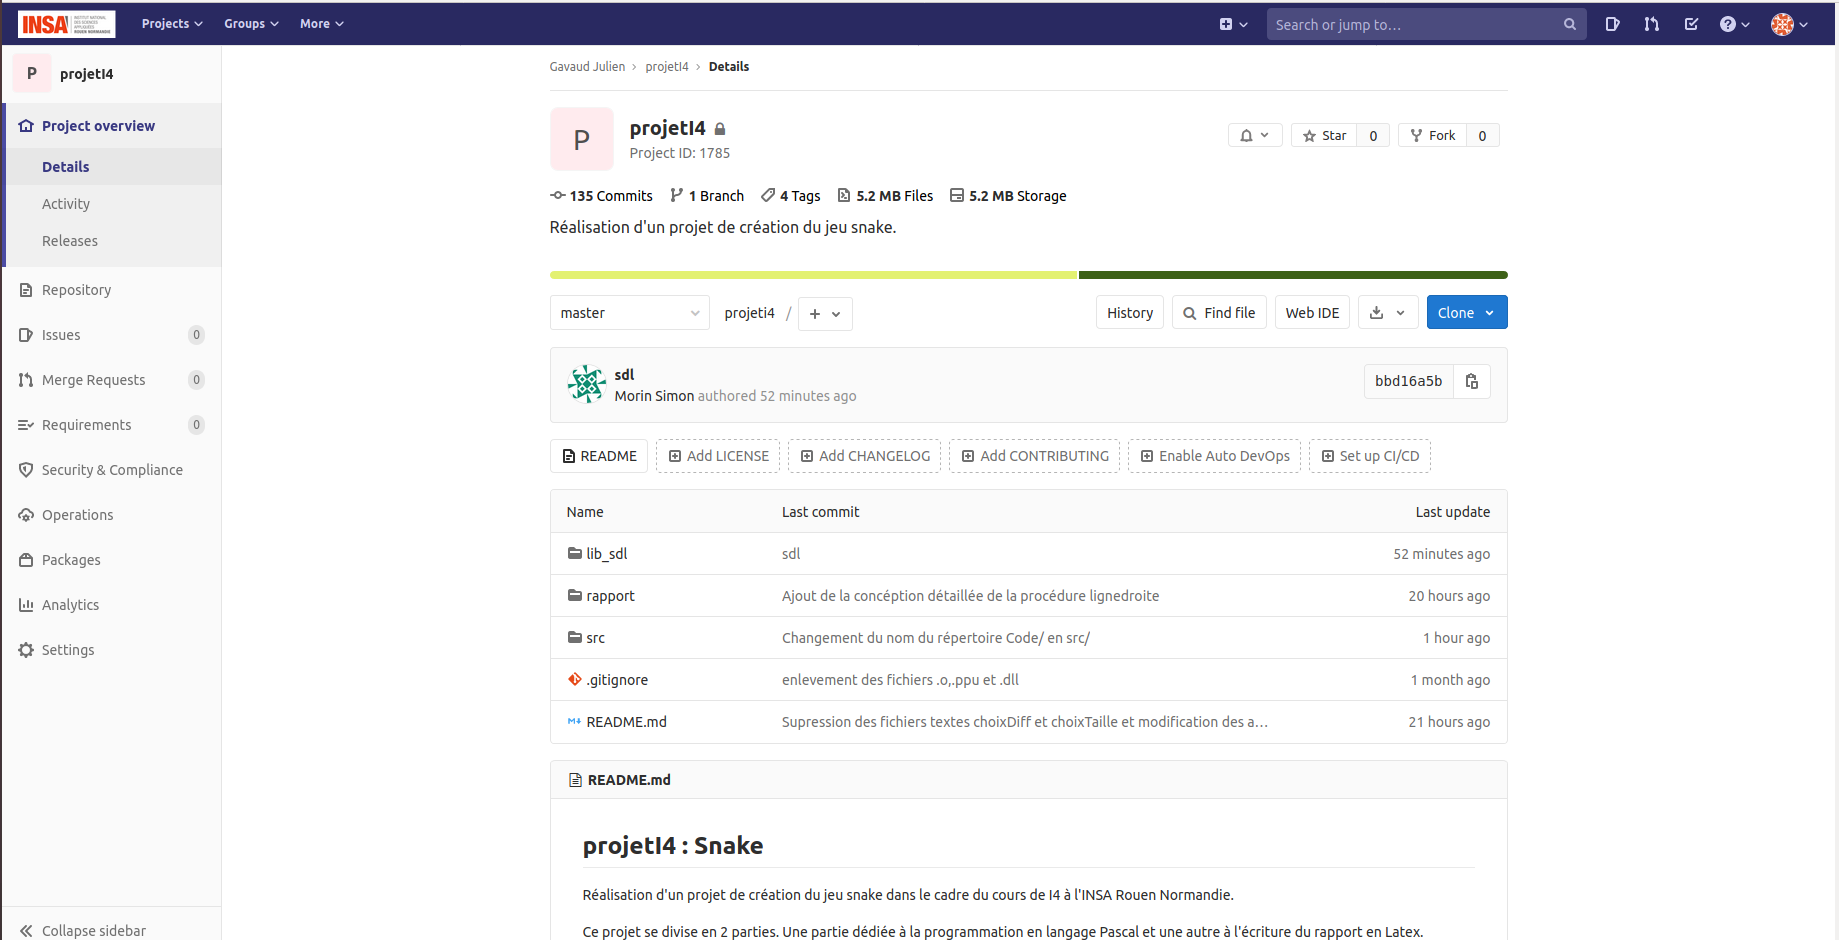
\includegraphics[width=1\textwidth]{images/depot_GitLab.png} 
            \caption{Dépôt GitLab.}
            \label{Dépôt_GitLab}
            
        \end{figure}
        
        \clearpage
        
        \subsection{Travail de groupe}
            L'intérêt de GitLab est donc de faciliter la travail de groupe. Chaque membre peut apporter sa contribution au projet, au moment où il le souhaite, et partager facilement son travail sans avoir à s'échanger des documents par mail ou autre.
        
            \subsubsection{Répartition des tâches}
                La répartition des tâches à été réalisée au bout de la troisième semaine de TD. En effet, au début, nous réfléchissions à la structure du programme tous ensemble et nous écrivions le cahier des charges du projet. Après avoir défini les grandes lignes du projet et consulté M. Baert, nous avons décidé de nous répartir les tâches pour être le plus efficace possible. La répartition s'est faite en fonction des envies et des compétences de chacun. Kevin Gatel et Simon Morin ont principalement travaillé sur le codage Pascal tandis que Julien et Théo ont codé quelques procédures Pascal mais ont plus travaillé à coder le rapport en \LaTeX. Bien évidemment, nous nous réunissions régulièrement par visio-conférence pour travailler ensemble et faire des points sur l'avancement du projet. Malgré le confinement, nous n'avons pas eu de mal à travailler ensemble grâce à Discord où nous pouvions partager nos écrans pour travailler à plusieurs. 
                
                Les deux derniers membres du groupe Hengshuo et Yizhen n'ont pas participé au projet, notament car nous n'avons eu aucun contact avec eux depuis le confinement. Nous comprenons les difficultés liées à celui-ci et à l'éloignement géographique mais nous avons été étonné de ne recevoir aucune réponse à nos nombreux messages, ne serait-ce que pour savoir s'ils pouvaient et/ou comptaient nous aider.
        
            \subsubsection{Retour d'expérience}
                Il paraît évident que nous avons rencontré plusieurs difficultés au cours de ce projet, que ce soit par rapport à l'algorithmique, au codage en \verb|Pascal|, en \verb|Latex| ou bien lors de l'utilisation de \verb|GitLab|.
            
                \paragraph{Algorithmique et Pascal} 
                    C'est la création des procédures gérant les fonctions de déplacement du serpent qui nous ont demandé le plus de réflexion. C'est le cœur du jeu et nous voulions que les déplacements soient le plus fluide possible. Au début du projet, nous travaillions avec des variables tête et queue qui étaient des coordonnées et corps qui était un tableau de type coordonnée. Comme le code était laborieux, nous avons décidé de redéfinir nos types et de créer un seul tableau comprenant toutes les coordonnées. Cela nous a fait changer beaucoup de choses dans notre projet qui était déjà bien avancé mais c'était nécessaire. 
                    Les délais d'apparition des pommes et des pommes dorées n'ont pas été faciles à programmer non plus. Nous voulions que la durée soit la même peu importe la vitesse du serpent et ça sans utiliser la fonction \verb|GetTime|. 
                    
                    Dans l'ensemble, ce projet nous a fait progresser en algorithmique. Nous nous sommes aussi rendu compte que nous avons encore de grosses marges de progressions. La prochaine étape est d'utiliser les pointeurs qui nous auraient sûrement permis d'obtenir un rendu encore meilleur. 
            
                \clearpage
                
                \paragraph{Git} 
                    Tout d'abord, lors de la première séance, nous avons modifié nos noms sur la page de garde et utilisé les mêmes lignes de texte. Ainsi, des merges apparaissaient et cela nous a permis de comprendre le fonctionnement de ce logiciel et les problèmes que nous allions pouvoir rencontrer. Celui-ci effectue une fusion des deux versions entrées en remplaçant les lignes modifiées par les utilisateurs. Seulement, si deux lignes sont toutes les deux modifiées, nous rencontrons un problème de merge. Pour résoudre ce merge nous devons modifier manuellement les lignes d'erreur. Ce problème a été assez difficile à gérer lors des premières séances. Nous ne comprenions pas comment fusionner les documents et résoudre les merges.
            
                    Néanmoins, au fur et à mesure, nous avons réussi à résoudre ces erreurs assez facilement. Nous nous organisions également pour ne pas travailler en même temps sur les mêmes choses pour éviter ces problèmes. 
            
                    Nous avons réellement essayé de nous approprier le service GitLab. Nous avons par exemple créé des clés ssh pour ne plus  avoir à nous connecter à chaque push/pull. Nous avons créé des issues sur GitLab ce qui permet de s'organiser sur les tâches restantes. GitLab possède de nombreuses fonctionnalités qu'il nous reste encore à découvrir lors de prochains projets.
            
                \paragraph{Rapport et \LaTeX}
                    Le langage d'écriture que nous avons utilisé est le \LaTeX. Cette écriture permet une présentation propre et soignée. L'avantage du \LaTeX est de permettre à l'utilisateur de se concentrer sur le contenu et non sur la forme. La mise en page est définie une fois au début du projet (ici fournie dans le document \textit{classeRapport}) et ensuite, c'est automatique. Cet aspect nous a beaucoup plu, car nous sommes tous d'accord pour dire qu'un des passages les plus pénibles lors de l'écriture d'un rapport est la mise en page. Une des grandes forces du \LaTeX est également le rendu des équations mathématiques et des algorithmes. Nous avons découvert cela pendant ce semestre et d'autant plus grâce au confinement et les cours à distance. C'est une découverte qui va nous servir pour la suite car écrire des formules sur \verb|Word| n'est pas l'idéal ... 
                    
                    Pour ce qui est des algorithmes le rendu est très satisfaisant, mais leur écriture n'est pas aisée. Nous avons eu des difficultés avec le package \verb|Algorithm2e|. Par exemple, un algorithme faisant plus d'une page "disparaît" à la fin de celle-ci sans s'écrire sur la suivante. Malgré nos recherches nous n'avons pas trouvé de moyens de résoudre ce problème. 
                    L'apprentissage est donc au début complexe, il existe une variété de commandes élévée. Nous avons souvent eu le sentiment de ne pas pouvoir profiter pleinement des possibilités qu'offre le \LaTeX. Rien que d'insérer une image sur la page de garde nous a posé problème. Les indications pour résoudre les problèmes de compilation ne sont pas toujours explicites et cela prend souvent du temps avant de trouver ce qui ne va pas. Par exemple, nous avons cherché pendant près d'une heure pourquoi le rapport ne compilait pas, pour se rendre compte que l'erreur venait d'une majuscule manquante (pour écrire le mot \LaTeX "stylisé" et pas Latex). 
            
                    Seulement, après de nombreuses heures de pratique, cela devient plutôt rapide et permet un rendu de qualité. Le \LaTeX n'est pas facile à prendre en main, mais une fois que l'on a fait cet effort on y voir réellement de nombreux avantages.

                    \clearpage
                    
                    Nous avons utilisé deux éditeurs de texte différents : 
                    
                \begin{itemize}
                    \vspace{0,2 cm}
                    
                    \item Kile pour Kevin, Simon et Julien. Kile est un éditeur minimaliste et peut se montrer assez destabilisant lors des premières utilisations.
                    \item Overleaf pour Théo. Son utilisation est simple et la page est assez design. De plus, je réutiliserai ce compilateur de \LaTeX car les erreurs de compilation empêche rarement la création du pdf. 
                    
                    \vspace{0,2 cm}
                \end{itemize}

            \par
                Néanmoins, des erreurs de compilation pouvait apparaître lors d'un passage à l'autre entre les éditeurs, ce qui était parfois ennuyeux.
                
            \subsubsection{Avis sur Git}
                \begin{itemize}
                    \item Théo : \enquote{GitLab est pour moi un excellent outil pour rassembler tout les codes sources, que ce soit du \LaTeX ou du Pascal. Les commandes utilisés à partir du Terminal permettent une utilisation fluide et rapide. On peut ainsi facilement voir les avancées qui ont été réalisées par les autres membres, via le 'poids' de chaque modification. Seulement, les problèmes de merge nuisent énormément à ce système. En effet, il faut alors soit écrasé une des deux parties, soit passer un temps fou à reprendre à la main. La gestion automatique des problèmes de fusion des fichiers ou une interaction simplifié avec l'utilisateur rendrait le logiciel bien plus utile et indispensable.}
        
                    \vspace*{0,4 cm}
        
                    \item Julien : \enquote{J'ai vraiment apprécié la découverte du logiciel Git. Une fois la prise en main effectuée j'y vois de réels avantages. Bien que je ne veuille pas aller en ASI/ITI, je pense que Git pourrai me servir dans le futur pour des rapports écrits (en \LaTeX ou autres). Le problème est que je me demande si je pourrai réutiliser le logiciel étant donné que la majorité des personnes ne connaissent pas Git. Concernant le \LaTeX, j'apprécie le rendu et les possibilités qu'offre le langage mais je ne pense pas le réutiliser sous la forme de code source dans un futur proche. En revanche, cela me donne envie d'utiliser des logiciels comme LyX.}
        
                    \vspace*{0,4 cm}
        
                    \item Kevin : \enquote{Gitlab est une plateforme en ligne permettant de synchroniser nos fichiers. Il a été d'une grande utilité notamment grâce à son utilisation assez simple et rapide, les fichiers communs sont modifiés simplement grâce à quelques lignes de commande sur le terminal. Le simple bémol serait sur les petits problèmes survenant un peu aléatoirement, nous obligeant à recloner le projet. Dans l'ensemble gitlab m'a convaincu et je l'utiliserai de nouveau pour un projet futur.}
        
                    \vspace*{0,4 cm}
        
                    \item Simon : \enquote{Je pense que GitLab est très pratique pour stocker et partager des fichiers. Il permet de synchroniser rapidement le contenu de nos dossiers, avec le dépôt en ligne, sans perdre de temps à devoir créer des archives et à se les transférer entre membres du projet. Il permet aussi de voir en ligne les modifications faîtes, de commenter des lignes de codes pour l'améliorer, et de créer des 'tâches' pour résoudre des problèmes, ce qui est plutôt cool. Le plus important est de ne pas partager un code source qui ne compile pas sinon une partie du dépôt est corrompue et c'est la croix et la bannière pour corriger les erreurs (surtout si c'est une autre personne qui a écrit le code).}
        
                \end{itemize}
                
                \clearpage



    \clearpage 
    \vspace*{\stretch{1}}
    
        \section*{Conclusion}
        \addcontentsline{toc}{section}{Conclusion}
        
        Au cours de ce projet, chaque membre du groupe a pu développer ses compétences informatiques et organistationnelles. Nous sommes contents du résultat et du travail que nous avons fourni. Malgré les conditions particulières dans lesquelles ce projet a été mené, nous avons réussi à travailler ensemble et à mettre nos compétences en commun pour mener à bien ce projet. Ces conditions ont démontré l'efficacité et la fiabilité de la méthode de travail apprise lors de ce cours. L'outil Git a permis une bonne organisation et nous sommes tous d'accord pour dire qu'il nous a grandement facilité le travail. Nous avons également découvert le \LaTeX lors de ce projet. Nous sommes conscients des avantages qu'il offre mais étant donné sa relative compléxité il nous faudra encore de l'entraînement avant de pouvoir en tirer réellement des bénéfices. 
 \vspace*{\stretch{1}}

        \clearpage

        
        \section*{Sources}
        \addcontentsline{toc}{section}{Sources} 
            \begin{itemize}
                \item Photo de la page de garde: \url{www.tuitec.com/lemblematique-jeu-snake-est-de-retour-sur-messenger/}
                \item Photo du logo GitLab page~\pageref{logo_GitLab}: \url{https://upload.wikimedia.org/wikipedia/commons/e/e1/GitLab_logo.svg}
                \item Photo du logo du logiciel Git page~\pageref{logo_Git}: \url{https://blog.syloe.com/wp-content/uploads/2014/12/git-logo-.jpg}
            \end{itemize}

\end{document}
